\chapter{Konzeption}

 \section{Bewertungskriterien}
 
 Im folgenden Kapitel werden drei Lösungsalternativen zur mobilen Aufmaßerfassung aus dem Google Play-Store anhand der erweiterteten Nielsen-Heuristiken \todo{ref} bewertet und verglichen.
Hierzu werden die Heuristiken zunächst kurz vorgestellt, und anschließend iterativ auf die Apps angewendet. Die für den Einsatzbereich des Gerüstbaus am Wichtigsten Kriterien werden abschließend in einer vergleichenden Tabelle zusammengetragen, um einen guten Überblick über die Testergebnisse zu schaffen. \\

 Diese drei ausgewählten Apps waren bei der Suchanfrange nach ``Aufmaßerfassung'' im Play-Store die am best bewerteten (Stand Januar 2018)
 \todo{Bild vom play-store} \\
 \subsection{Erweiterte Nielsen-Heuristiken}
1990 entwickeln Rolf Molich und Jakob Nielsen neun Usability-Heuristiken, die auf einer Grundlage von allgemein anerkannten Prinzipien beruhen. 4 Jahre später ergänzt Nielsen diese um einen zehnten Punkt: 

\begin{enumerate}
	\item \label{1} Sichtbarkeit des Systemzustands
	\item \label{2} Übereinstimmung zwischen System und realer Welt
	\item \label{3} Benutzerkontrolle und -freiheit
	\item \label{4} Konsistenz und Standards
	\item \label{5} Fehlervorbeugung
	\item \label{6} Wiedererkennung statt Erinnern
	\item \label{7} Flexibilität und Effizienz der Benutzung
	\item \label{8} Ästhetisches und minimalistisches Design
	\item \label{9} Erkennbarkeit, Diagnose und Erholung von Fehlern
	\item \label{10} Hilfe und Dokumentation
\end{enumerate} 

Zur Bewertung mobiler Endgeräte reichen diese zehn Bewertungskriterien jedoch nicht vollständig aus, sodass weitere 8 Heuristiken, die speziell für mobile Geräte ausgelegt sind, hizugezogen werden \todo{ref auf ue, 239}

\begin{enumerate}
	\setcounter{enumi}{10}
	\item \label{11} Adäquater Umgang mit Unterbrechungen
	\item \label{12} Fokussieren der Informationen
	\item \label{13} ``Joy of Use''
	\item \label{14} ``Don't lie to the user''
	\item \label{15} Unterstützung verschiedener Bildschirmorientierungen
	\item \label{16} Ergonomische Gestaltung der physischen Interaktion
	\item \label{17} Einfache Eingabe, Bildschirmlesbarkeit und Übersichtlichkeit
	\item \label{18} Schützen der Privatsphäre
\end{enumerate}

\subsection{Weitere Kriterien}
Zusätzlich werden die Lösungs-Alternativen mit 2 weiteren Kriterien bewertet, die für die Benutzung zur mobilen Aufmaßerfassung im Gerüstbau wichtig sind:

\begin{itemize}
	\item Integration der Software-Lösung in die bereits vorhandene App der Fa. VERO
	\item Export des Bildes und der Metadaten zur Weiterverarbeitung in einem nachgeschalteten Dienst (API)
	\todo{mehr Kriterien raussuchen}
\end{itemize}

\section{Bewertung vorhandener Lösungalternativen}

Im Folgenden werden die 3 Alternativen nacheinander mit Hilfe der oben genannten Heuristiken/Kriterien bewertet, und abschließend ein vergleichendes Fazit in Form einer Tabelle \todo{ref auf tabelle?} gezogen.

\subsection{Photo Measures}

\textsc{Photo Measures} von Big Blue Pixel Inc. VERSION, RATING \todo{link zum Playstore} \\

\begin{wrapfigure}{R}{0.4\textwidth}
	\centering
	\includegraphics[keepaspectratio, width=0.4\textwidth]{photo_measures/help}
	\caption{Initialer Start}	
	\label{fig:pmhelp}
\end{wrapfigure}

Die App zeigt beim ersten Start ein helfendes Overlay, welches dem Nutzer genau erklärt, wie die App zu benutzen ist. Dieser Punkt fällt nach Nielsen unter \ref{10} (Siehe Abbildung\ref{fig:pmhelp}) \\
 
Aktionen sind nur dann verfügbar, wenn sie benutzbar sind. Somit werden Fehler vorgebeugt, und der Benutzer weiß zu jeder Zeit, in welchem Systemzustand er sich befindet. Dies korrespondiert zu den Heuristiken~\ref{1} und \ref{5}. \todo{2 bilder mit bottom-bars} \\

Die App bedient sich einer Reihe universell bekannter Icons, sodass intuitiv erkennbar ist, welche Aktion sich hinter welchem Button verbirgt, ohne groß darüber nachdenken zu müssen. Zusätzlich stehen die entsprechenden Aktionen als Text unter den Icons. Dies kann nützlich sein, wenn ein Icon nicht auf Anhieb wiedererkannt wird. \ref{4} \todo{ref auf pic von bottom-bars} \\

Des Weiteren gibt die App dem Benutzer die Möglichkeit, Formen, Größen und Farben anzupassen. Dies fördert eine flexible und effizente Benutzung. \ref{7} \\

Ein durchaus schwerwiegender negativer Punkt liegt bei der Benutzerkontrolle \ref{3} der App. So ist es dem Benutzer nicht möglich, über einen Undo- bzw. Redo-Button seine Aktionen zu revidieren. Dies ist gerade bei der Bearbeitung von Bildern, wo es viele aneinandergereihte Aktionen des Benutzers gibt, eine entscheidende Funktionalität, welche nicht nur die Gedächtnisbelastung des Benutzer senken, sondern auch den ``Joy of Use'' deutlich steigern kann. \\

Zudem bietet die App keine für den Nutzer erkennbare Ausstiegsmöglichkeit \ref{6} an. Es gibt weder einen Zurück-Button, noch einen Button um das annotierte Bild explizit zu speichern. Die einzige Ausstiegsmöglichkeit erfolgt über die Zurück-Navigationstaste des Smartphones, welche das Bild auch zusätzlich speichert. Diese Lösungsvariante ist für den Nutzer nicht intuitiv verständlich. \todo{bild}

Die App erfüllt nahezu alle acht (\ref{11}-\ref{18}) Heuristiken für mobile Geräte. Zu jeder Zeit ist auf dem Bildschirm erkennbar, welche Form zur Zeit ausgewählt ist. Das Smartphone kann während der Benutzung pausiert bzw. gedreht werden, ohne dass Informationen verloren gehen, oder der Benutzer durch unbekannte Bausteine überrascht wird. \todo{screens} Hier fällt als einziger negativer Punkt die unzureichende Gesten-Unterstützung auf \ref{13}. So malt der Benutzer unabsichtlich mit jeder Zoom-Geste eine Form in das Bild, welche danach wieder gelöscht werden muss, da es keine Undo-Funktion gibt. \\

\subsection{Measuring Master}

\textsc{Measuring Master} von Robert Bosch GmbH VERSION, RATING \\

\begin{wrapfigure}{R}{0.4\textwidth}
	\centering
	\includegraphics[keepaspectratio, width=0.4\textwidth]{bosch/help}
	\caption{Zeichen-Modus}	
	\label{fig:bhelp}
\end{wrapfigure}

Die App zeigt in einer Art Statusleiste am unteren Rand des Bildschirms den aktuellen Modus an, und gibt über einen auffordernden Text am oberen Bildschirmrand dem Nutzer eine Hilfestellung, was er im gerade ausgewählten Modus machen kann. \todo{screens} Hiermit deckt die App Nielsen \ref{1} und \ref{10} ausreichend ab. \\

Des Weiteren benutzt auch diese App universell verständliche Icons, um die wichtigsten Aktionen wiedererkennbar zu machen. So hat beispielsweise das Mülleimer-Icon in jedem Modus die Löschfunktion. \\

Im Gegensatz zu \textsc{Photo Measures} bietet diese App dem Benutzer die Möglichkeit seine Aktionen rückgängig zu machen, oder sie zu wiederholen. Dies ist ein deutlicher Vorteil seitens der Usability, da Fehler nicht so hart bestraft werden, als wenn keine Undo/Redo-Button vorhanden wären. \\

Fehler werden hier durch das Deaktivieren von Buttons, die im aktuellen Systemzustand nicht benutzbar sind, präventiv verhindert. Das Löschen von Formen ist beispielsweise nur dann möglich, wenn zuvor eine Form ausgewählt wurde.

Negativ fällt auch in dieser Alternative die fehlerhafte Gesten-Unterstützung auf. So sorgen Zoom-Gesten per Doppel-Tap zum unabsichtlichen Zeichnen einer Form, welche im Nachhinein wieder gelöscht werden muss. Außerdem verletzt die App Nielsen~\ref{15}, da Änderungen in der Bildschirmausrichtung dafür sorgen, dass das Bild nicht wie erwartet seine Ursprungsausrichtung beibehält, sonder auch rotiert wird. 

\begin{figure}[h]
	\begin{subfigure}[b]{0.5\textwidth}
		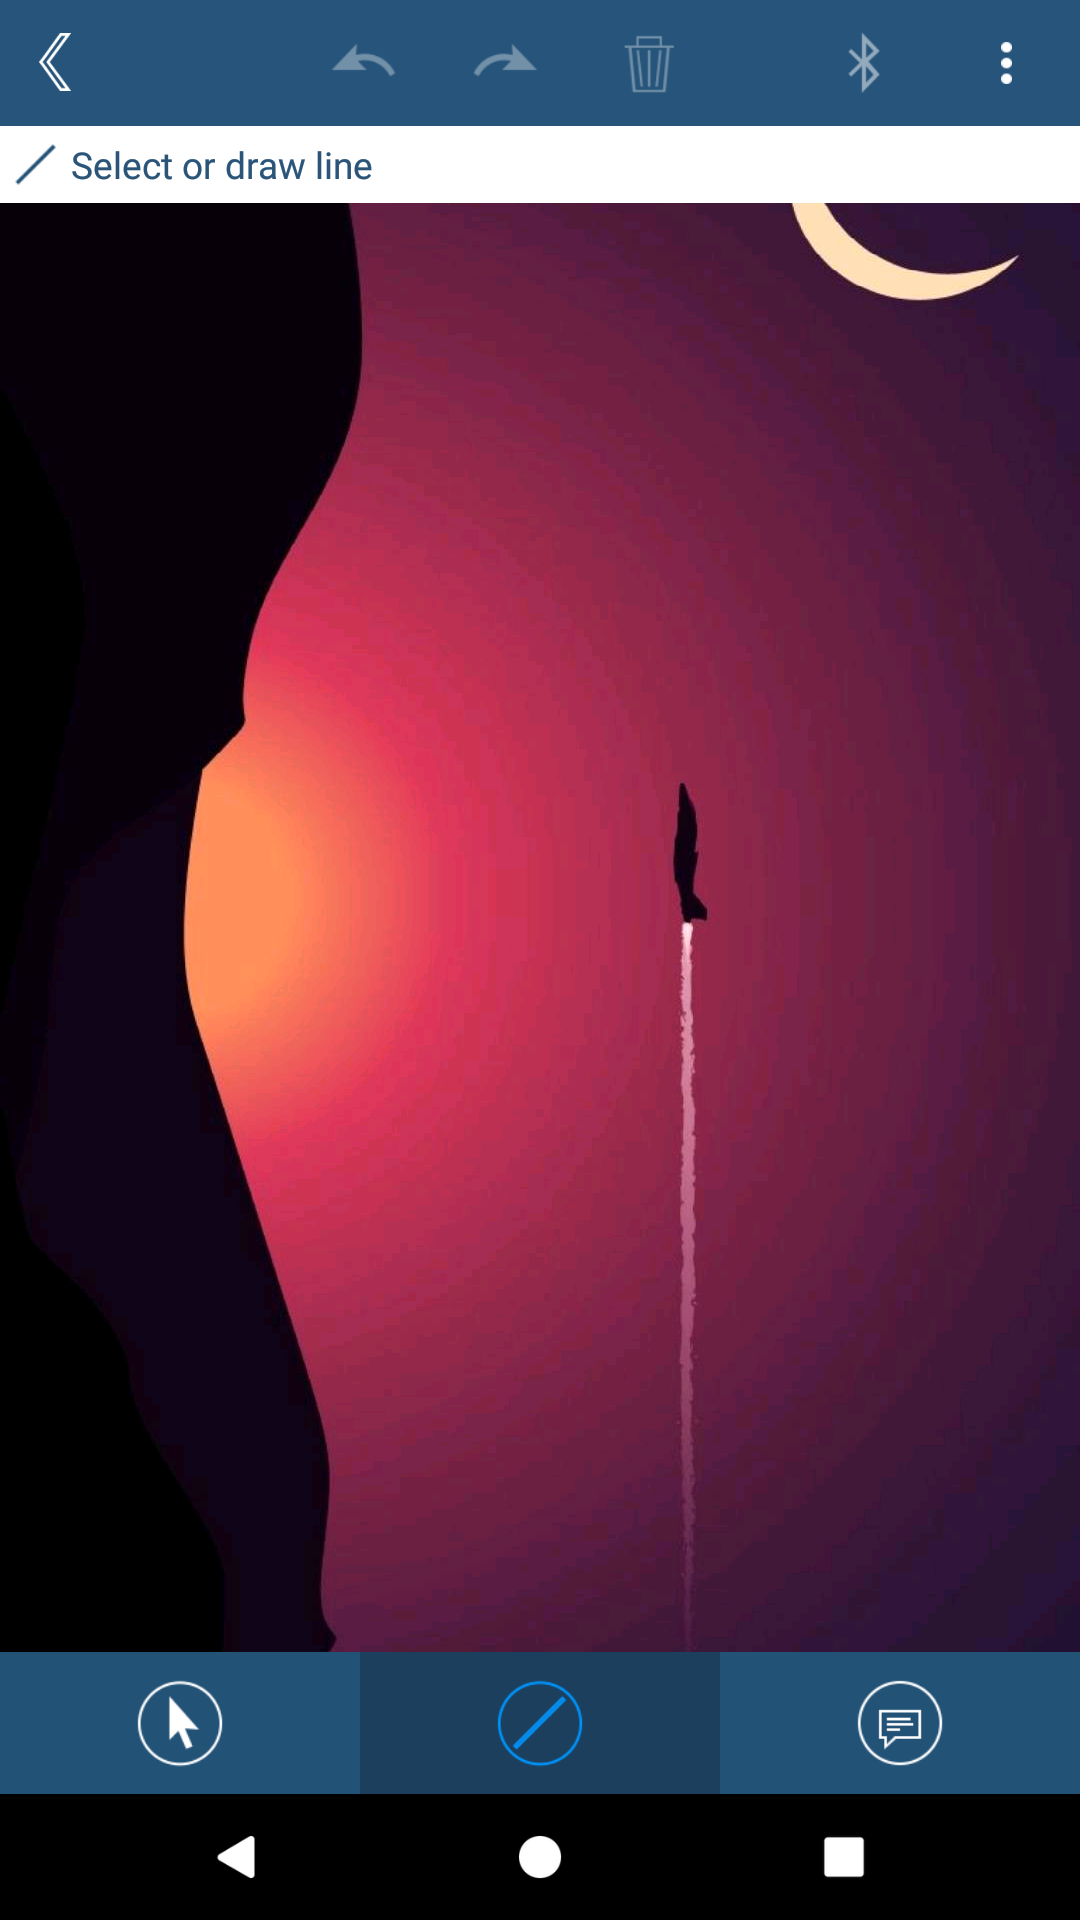
\includegraphics[keepaspectratio, width=0.9\linewidth]{bosch/portrait}
		\caption{App im Portrait-Modus}
		\label{fig:bportait}	
	\end{subfigure}
	~
	\begin{subfigure}[b]{0.5\textwidth}
		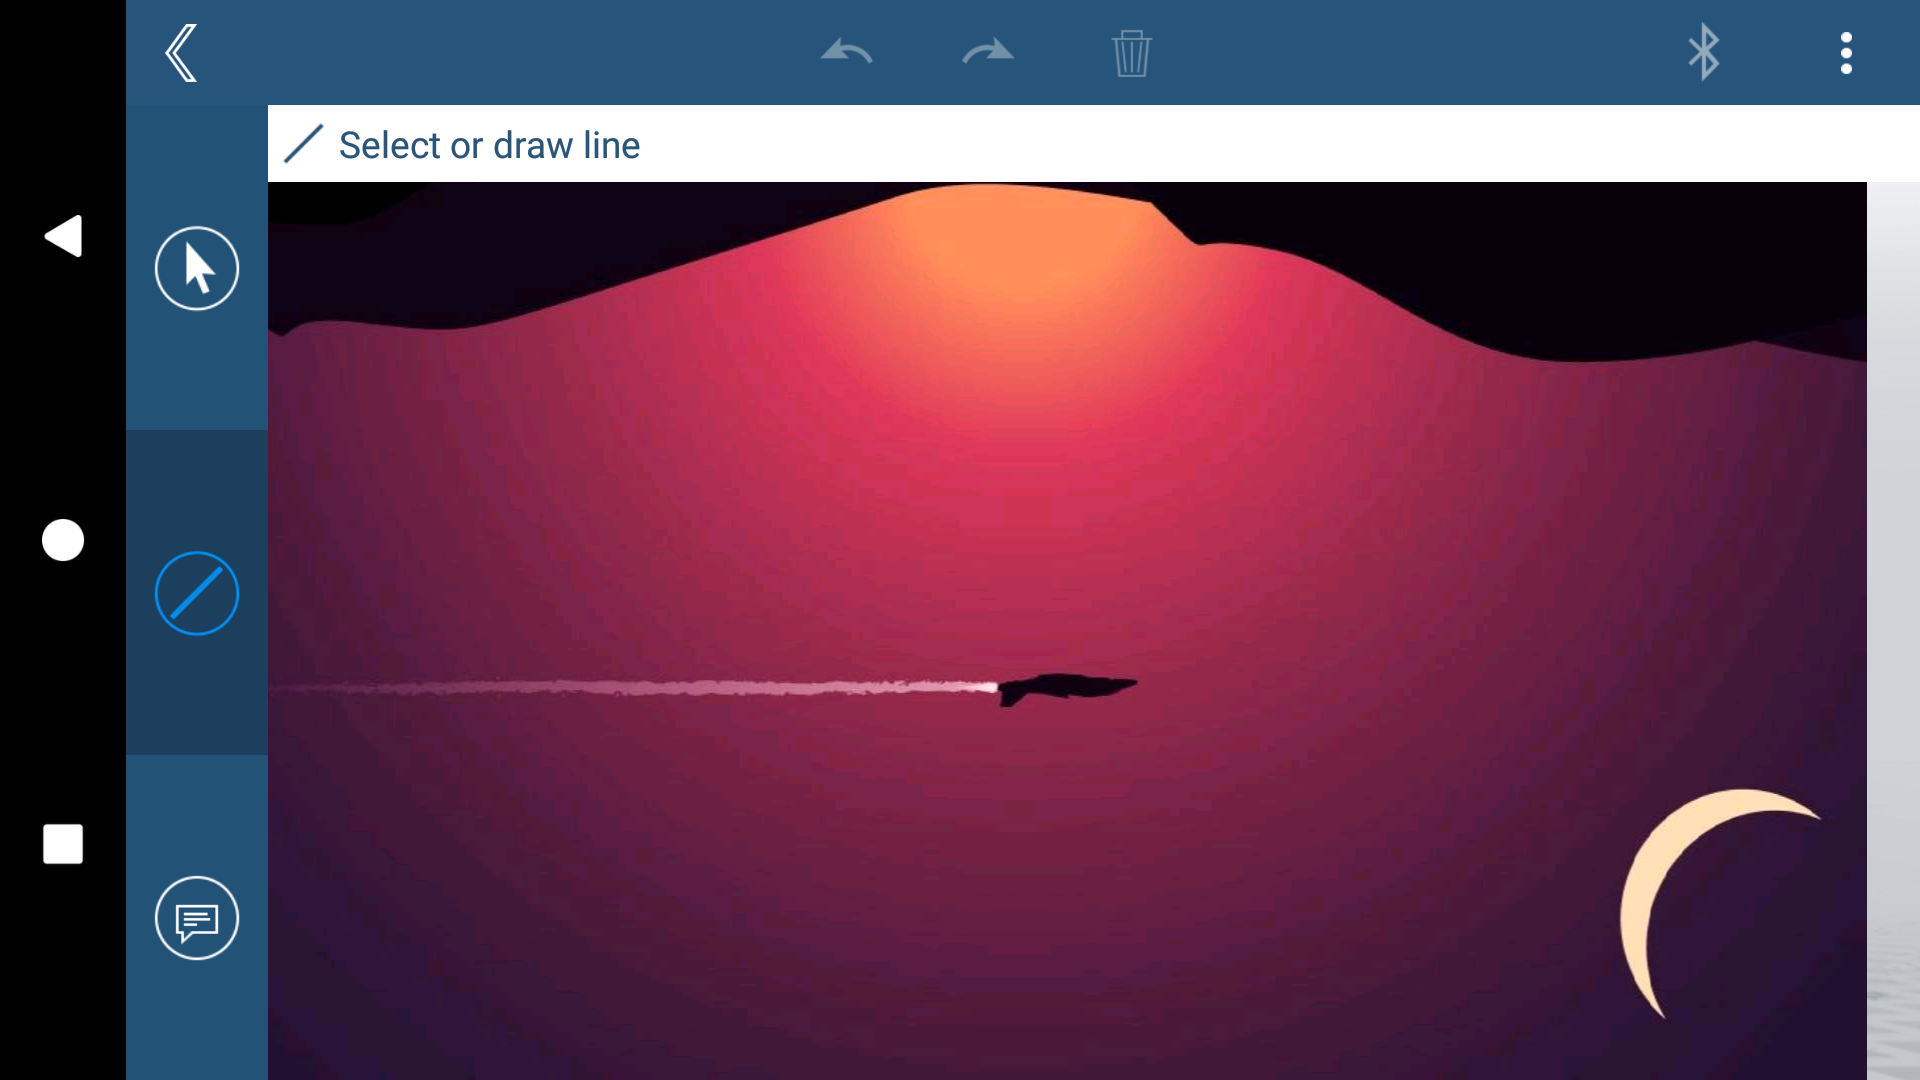
\includegraphics[keepaspectratio, height=0.7\linewidth]{bosch/landscape}
		\caption{App im Landscape-Modus}
		\label{fig:blandscape}	
	\end{subfigure}
	\caption{Bildschirmrotation Bosch-App}
	\label{fig:borientation}
\end{figure}

\section{Bewertung der Lösungsalternativen}
\section{Vorgehensweise bei Implementierung eigener Software-Lösung}
  \subsection{Iterativer Entwicklungsprozess}
    3 Iterationen jeweils Mitte Dezember, Januar und Februar \\
    Feedback in Form von Gitlab-Issues und Beobachten von Testpersonen (Usability-Experimente) \\
    1. Iteration (Dezember): App mit floating buttons (screenshots vorher-nachher)
    2. Iteration (Januar): App mit status bar (screenshots vorher-nachher)
    3. Iteration (Februar): App mit Help-Overlay \& verbesserter Statusbar (screenshots vorher-nachher)
  \subsection{8 Goldenen Regeln von Shneidman}
  \subsection{DIN und ISO-Normen}
  \subsection{Material Design-Guidelines}
  \subsection{ABC-Modell}
  \subsection{Gesture-Support (papers)}
    Zoom-Area und Panning am besten geeignet um Content auf kleinen Displays darzustellen \\


  
